\hypertarget{earlyexiting}{%
	\chapter{Edge Offloading with Early Exiting}\label{ch:edgeoffloading}}
\thispagestyle{fancy}

In this chapter we implement a edge-based offloading scheme utilizing early exiting \gls{dnn}s. Our scheme a more flexible and adaptive than currently proposed in literature. In section \ref{sec:edge-aee} we present our offloading scheme In section \ref{sec:edge-system-model} we define the system model used to evaluate our result. We describe our implementation in section \ref{sec:edge-implementation} In section \ref{sec:edge-exp-setup} we describe our experimental setup. In section \ref{sec:edge-results} we present our results and in section \ref{sec:edge-summary} we discuss our results.

\section{\acrfull{aee} for Time-Critical Applications} \label{sec:edge-aee}

We propose \acrfull{aee} an optimistic standalone inference model based on early exit \gls{dnn}. It is optimistic in the sense, that it allows the edge server to reach as far as possible in the inference process before time is out. The early exits or in this case intermediate classifiers, as we do not exi, but continuously send back increasingly confident predictions. We argue, that \gls{aee} will in any case achieve at least the same accuracy as upfront exit selection in \cite{li_edge_2018}, even though the exit have been chosen with care, the risk of timeout is still present as both computation and communication delays are not constant. If unexpected delays do occur, it may cause timeouts and lead to lost predictions. However, our scheme reduces the risk of losing prediction by timeout, if an earlier, albeit less accurate predictions is available. 

\begin{figure}
	\captionsetup[subfigure]{justification=centering}
	\centering
	\subfloat[Continuois predictions\label{fig:offloading-scheme-successful}]{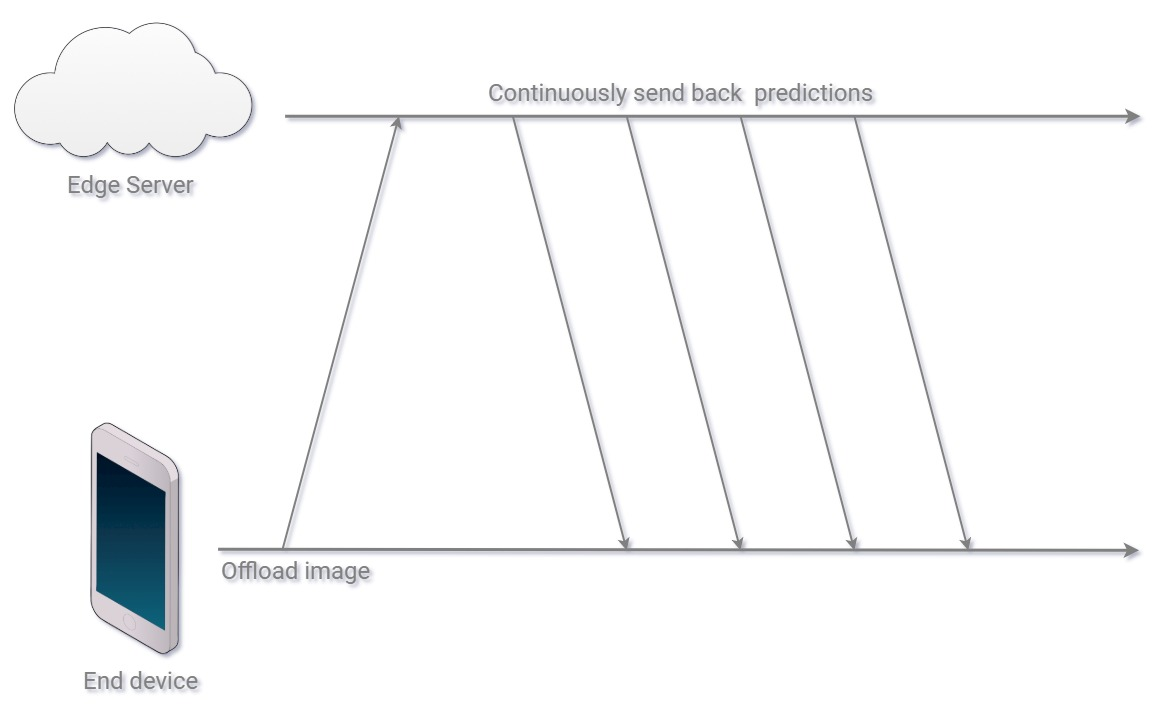
\includegraphics[width=.7\linewidth]{figures/models/timeline_all}}
\end{figure}
\begin{figure}
		\captionsetup[subfigure]{justification=centering}
	\centering
	\subfloat[Timeout of Continuois predictions\label{fig:offloading-scheme-timeout}]{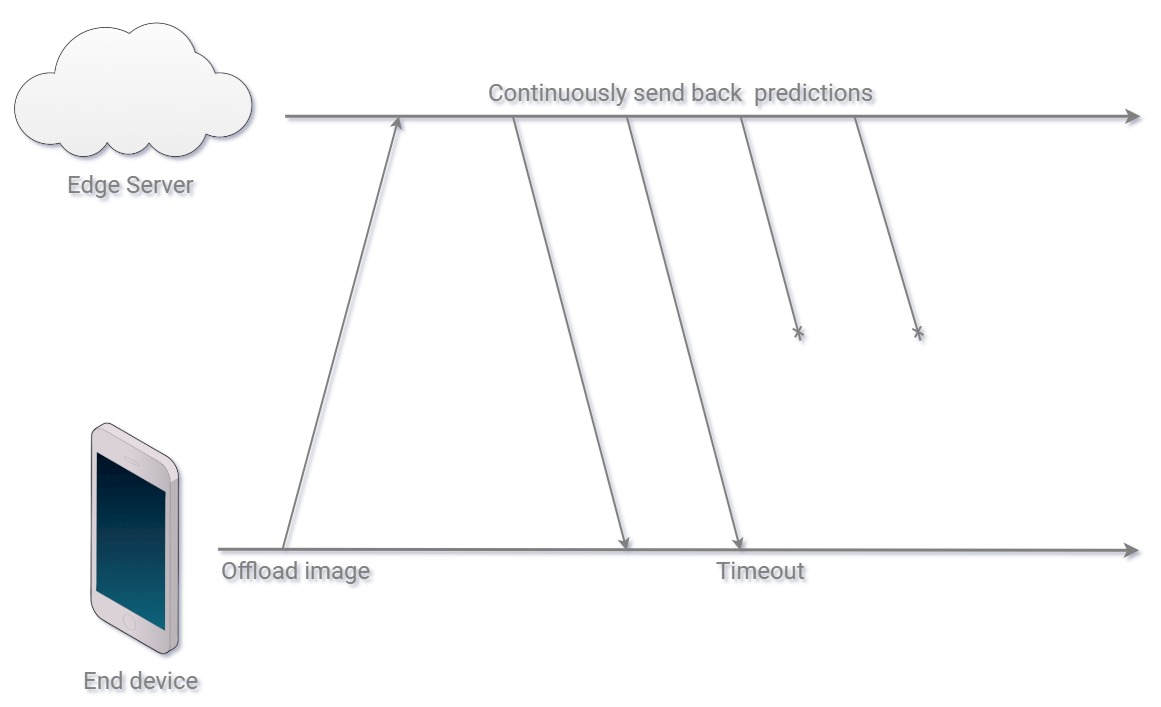
\includegraphics[width=.7\linewidth]{figures/models/timeline_timeout}}
	\caption[Offloading scheme]{offloading scheme}
	\label{fig:offloading-scheme}
\end{figure} 

Figure \ref{fig:offloading-scheme} illustrates the offloading scheme. To not waste idle time on edge server the data is immediately offloaded from the end device, to edge server. The edge server preprocesses the data, runs the \gls{dnn} inference process, and whenever a prediction is obtained from the early ecit \gls{dnn}, a thread is spawned to send back the result to the end device. Multiple early exits allows for successively receiving, what is expectedly, increasingly reliable predictions. Figure \ref{fig:offloading-scheme-successful} illustrates the continuous reply of predictions. Figure \ref{fig:offloading-scheme-timeout} illustrates a case, where a timeout occurs and only two predictions are available 

The most recent received prediction i.e. from the latest exits are accepted as the prediction. Or alternatively, we also look at using multiple predictions received from the edge, and let the end device use the information to select the prediction using a combination function, defined in section \ref{sec:edge-system-model}.

\section{System Model} \label{sec:edge-system-model}

In this section we define the system model for \gls{aee}. Note the metrics defined in chapter \ref{ch:earlyexit} is reused. To remind the reader:  $ C $ denotes the number of the image classes, $ N $ denotes the number of the exit points in a DNN, $ I $ denotes the number of images. 

We still do not differentiate between early exit and conventional model,  as we still use $ T_{i,n}^{cmp} $ to denote computation time irregardless of conventional inference model with a single exit, or early exit models with multiple. We do extend our view on latency, as we introduce two execution schemes.
	
	\begin{enumdescript}
		\item[Latency]  We have two options $ \left.A \right) $ local processing and $ \left.B\right) $ edge offloading. Hence we denote the computation time for local processing $ T_{i,n}^{loc,cmp} $ and $ T_{i,n}^{edge,cmp} $ to denote computation time at the edge. 
	
		
		We define the time for local and remote execution

		\begin{enumdescript}
			\item[Local Execution] If the classification exits from exit point $ n $, the processing delay of image $ i $ at local is presented as
			\begin{align}
			T_{i,n}^{loc}= T_{i,n}^{cmp,loc}
			\end{align}
			\item[Remote Execution] If the classification exits from exit point $ n $, the processing delay of image $ i $ at edge is presented as
			\begin{align}
			T_{i,n}^{edge}=T_{i}^{com}+ T_{i,n}^{cmp,edge}
			\end{align}
			where $ T^{com}_i $ denotes the communication time, for both uplink time to transmit image $ i $ from local to edge, and downlink time of prediction reply from edge to local.
			
			Offloading for remote execution is only sensible whenever we save time compared to local execution
			\begin{align*}
					T_{i,n}^{loc} > T_{i,n}^{edge}
			\end{align*}
			Due to the difference in computing resources, we expect the computation time at edge to be significantly lower than local computation time, i.e. $ T_{i,n}^{loc,cmp} > T_{i,n}^{edge,cmp} $. Thus, the communication time $ T^{com}_i $ becomes an important factor for offloading decision.

		\end{enumdescript}
	
		\item[Accuracy] The scheme opens the opportunities to receive multiple predictions within the time frame. We may be able to improve the accuracy and reduce undesired overthinking using the output results of the first $ n $ exit points to combine the information.
		
		\begin{align}
		\bar{A}_f &= 1 - \frac{1}{I} \sum_{i=1}^{I}\mathbb{I}\left(\left|f\left(\mathbf{\hat{c}}_{i,1} \dots, \mathbf{\hat{y}}_{i,n}\right)-y_i\right|\right)
		\end{align}
		
		remember the ground truth class label of image $ i $ and $ c_i \in \left[1, C \right] $ and $ \mathbb{I(\cdot)}  $ is a indicating function defined by
		\begin{align}
		\mathbb{I}(a)= \begin{cases}
		0, & \mathrm{if\:} a \leq 0, \\
		1, & \mathrm{otherwise}
		\end{cases}
		\end{align}
		
		There are several ways to define combination function $ f\left(\mathbf{\hat{y}}_{i,1}, \dots, \mathbf{\hat{y}}_{i,n}\right) $
		\begin{enumdescript}
			
			
			\item[Latest] We define the method \emph{lastest}, where we constrain ourselves to only use the most recent prediction $n$.
			\begin{align}
			f\left(\bm{\hat{y}}_{i,1}, \dots, \bm{\hat{y}}_{i,n} \right) = \hat{c}_{i,n}^{*}
			\end{align}
			
			\item[max confidence] This method used in \cite{kaya_shallow-deep_nodate}, reports improvement on the \gls{cifar10}, \gls{cifar100} and \gls{tinyimagenet}. The measure is based on the assumption, that an exit obtaining a higher score is more confident, hence improving the accuracy.
			\begin{align}
			\begin{split}
			f\left(\bm{\hat{y}}_{i,1}, \cdots, \bm{\hat{y}}_{i,n} \right) = \arg \underset{{\hat{y}_{i,j}^{*}, 1 \le j 
					\le n}}{\max} \{\hat{y}_{i,1}^* \dots, \hat{y}_{i,n}^*\},\\ \text{where\:} \hat{y}_{i,j}^* = \max\bm{\hat{y}}_{i,j} \text{\:for\:} \forall \ 1 \le j \le n
			\end{split}	
			\end{align}
			\item[sum confidence] this method sums the respective class scores for all exit predictions and chooses the highest scoring class. 
			\begin{align}
			\begin{split}
			f\left(\bm{\hat{y}}_{i,1}, \dots, \bm{\hat{y}}_{i,n} \right) = \arg \underset{n}{\max} \{s_{i,1}, \dots, s_{i,C}\}, \\ \text{where\:} s_{i,n} = \sum_{j=1}^{n}\hat{y}_{i,n,c} \text{\:for\:} \forall \ 1\le c \le C
			\end{split}
			\end{align}
			
			%				\item[weighted sum confidence] this method perform a weighted sums of the respective class scores for all exit predictions and chooses the highest scoring class. 
			%
			%				\begin{align}
			%				\begin{split}
			%					f\left(\bm{\hat{y}}_{i,1}, \dots, \bm{\hat{y}}_{i,n} \right) = \arg \underset{n}{\max} \{s_{i,1}, \dots, s_{i,C}\},\\ \text{where\:} s_{i,n} = \sum_{j=1}^{n}w_n \hat{y}_{i,n,c} \text{\:for\:} \forall \ 1\le c \le C
			%				\end{split}	
			%				\end{align}
			
			\item[max score margin] this method determines the score-margin for all exit predictions and chooses the class with the highest score-margin. 
			\begin{align}
			\begin{split}
			f\left(\bm{\hat{y}}_{i,1}, \dots, \bm{\hat{y}}_{i,n} \right) = \arg \underset{\hat{y}_{i,j}^{*}, 1 \le j 
				\le n}{\max} \{s^{*}_{i,1}, \cdots, s^{*}_{i,n}\},\\ \text{where\:} s^{*}_{i,j} = f_{margin}(\bm{\hat{y}}_{i,j}) \text{\:for\:} \forall \ 1 \le j \le n
			\end{split}	
			\end{align}
		\end{enumdescript}
	
		\item[Reliability]  We still define the reliability as in chapter \ref{ch:earlyexit}, as the fraction of samples, that can be correctly classified given a latency threshold $ \delta $.
		
		\begin{align}
		R= \bar{A} \cdot (1-\overline{F}^{to})
		\end{align}
		
		The timeout probability $ \overline{F}^{to} $ is also still defined as the number of samples not able to meet the delay requirement out of all samples in the set. However our latency is now not only dependent on local computation time.
		\begin{align}
		\overline{F}^{to}=\frac{1}{I}\sum_{i=1}^{I} \mathbb{I}\left(T_{i,n}-\delta\right)
		\end{align}
		Where
		\begin{align}
			T_{i,n} = \begin{cases}
				T_{i,n}^{loc} \\
				T_{i,n}^{edge}
			\end{cases}
		\end{align}
		We have a delay violation, if no prediction is provide and the execution time, no matter local or offloading is overrun, i.e. $ T_{i,n} > \delta $  
	
		\item[Problem formulation]   As in chapter \ref{ch:earlyexit}, we select exit point for each image and optimize its accuracy with a latency constraint. The inference time of image $ i $ at exit $ n $, cannot be greater than or equal to our latency threshold $ \delta $. However now we optimize our new accuracy, defined by the combination function
		
		
		\begin{maxi}
			{n}{\bar{A}^f_n}
			{}{}
			\addConstraint{T_{i,n}}{\leq \delta}
		\end{maxi}
		
		Exactly as in chapter \ref{ch:earlyexit}, we solve this problem,  using the best effort way, i.e., feed each exit results back and let user decide the prediction. For the same three reasons:
		\begin{enumerate}
			\item Computation latency uncertainty and now especially, that we offload, communication latency with a even higher degree of uncertainty, makes it hard to make decision in advance
			\item Upfront exit decision algorithm may take time
			\item Going through classifier of each exit point does not take too long time
		\end{enumerate}
		
			
	\end{enumdescript}  




%\begin{description}
%	
%	\item[Lastest prediction] We define the method \emph{lastest prediction}, where we constraint ourselves to only use the most recent prediction $n$. We do not need to do any class expansion nor to formulate the matrix $\mathbf{S}$. We only need to consider the first index of the vector $\mathbf{c}_{exit_n}$. The class label becomes our prediction $p$.
%	\begin{align*}
%	p = \mathbf{c}_{exit_n,0}
%	\end{align*}
%	Equivalently we could expand our score vector to $\mathbf{s^*}$ and find the argument of the maxima.
%	\begin{align*}
%	p = \arg \max \mathbf{s^*}_{exit_n}	
%	\end{align*}
%	Choosing the most confident prediction from the most recent result available, gives us the highest accuracy on average. However, we only use information form a single prediction, we might be able to formulate a mathematical function able to use information form multiple predictions to further improve the accuracy, as we have seen, that the later exit might make a correct prediction from an earlier exit incorrect. 
%	
%	\item[Confidence (max)] This method is based on the naive assumption, that given a higher score, it will lead to a higher accuracy independent of the uncertainty of classifier at an earlier exits. We use class expansion and  formulation our score matrix $\mathbf{S}$. From $\mathbf{S}$ we find the prediction $p$ as the argument of the maxima.
%	\begin{align*}
%	p = \arg \max  \mathbf{S}
%	\end{align*}
%	
%	\todo{How do I take first the row containing the max value, and then find the column/index of the maxium value?}
%	Here we neglect the fact, that the later exits are in general more accurate and assume, that a higher confidence despite the exit leads to a correct prediction and we do not account for the uncertainty introduces be less accurate exits.
%	
%	\item[Confidence (add)] We define a method, that additive combines information from all available predictions and selects the highest scoring class. The score vector are be expanded to the class space and represented as a matrix. We sum all columns of $\mathbf{S}$ to a 1-dimensional vector $s_{sum}$ of length $k$. 
%	
%	\todo{how to sum column of matrix?}
%	\begin{align*}
%	\mathbf{s}_{sum} &= \sum_{i=0}^{k} \mathbf{S}_{n,i}, \text{for\:} n=0, 2, \dots, j\\ 
%	&=	\begin{bmatrix}
%	s^*_0 & s^*_1 \dots & s^*_{k-1}
%	\end{bmatrix}_{1 \times k,\: k=100} 
%	\end{align*}
%	Our prediction becomes the argument of the maxima of $\mathbf{s}_{sum}$
%	\begin{align*}
%	p = \arg \max \mathbf{s}_{sum}
%	\end{align*}
%	
%	
%	\item[Confidence (add,weight)] Almost identical to \emph{confidence (add)}, but uses a weighted sum of all available exits to combine the information. Each exit are weighted to acknowledge the increasing accuracy as the predictions comes from a deeper exit in the model.  The weights can be represented by a column vector $\mathbf{w}$.
%	\begin{align*}
%	\mathbf{w}_{n} =
%	\begin{bmatrix}
%	w_0 &
%	w_1 &
%	\dots &
%	w_n
%	\end{bmatrix}^T
%	\end{align*}
%	The weights of row $n$ are multiplied all entries at row $n$ of $S$. Then we sum all columns of $\mathbf{S}$ to a 1-dimensional vector $s_{sum}$ of length $k$.  
%	\begin{align*}
%	\mathbf{s}_{ws} &= \sum_{i=0}^{k} w_n \cdot \mathbf{S}_{n,i}\\
%	&= 		
%	\begin{bmatrix}
%	s_0 & s_1 \dots & s_{k-1}
%	\end{bmatrix}_{1 \times k,\: k=100} 
%	\end{align*}
%	Our prediction becomes the argument of the maxima of $\mathbf{s}_{ws}$
%	\begin{align*}
%	p = \arg \max \mathbf{s}_{ws}
%	\end{align*}
%	
%	\item[Score-margin (max)] We use the score-margin, defined in \ref{}, to find the best prediction among the available predictions. We do not need to expand our score vector nor to formulate the score matrix. Instead we define a $n$-dimensional column vector, where row $n$ represent the score-margin at the corresponding exit-$n$.  
%	\begin{align*}
%	\mathbf{s}_{sm} = \begin{bmatrix}
%	\mathrm{ScoreMargin}(s_{0,0}, s_{0,1}) \\
%	\mathrm{ScoreMargin}(s_{1,0}, s_{1,1}) \\
%	\vdots \\
%	\mathrm{ScoreMargin}(s_{n,0}, s_{n,1})
%	\end{bmatrix}
%	\end{align*}
%	Our prediction becomes the argument of the maxima of the score-margin vector.
%	\begin{align*}
%	p = \arg \max \mathbf{s}_{sm}
%	\end{align*}
%	determines the score-margin between the two top-scoring predictions. We select the prediction from the exit with the highest score-margin. From the previous chapter, we know that the score-margin threshold gave a smaller proportion of incorrrectly exited samples at the small cost of samples, that could have been correctly classified using only highest scoring confidence.	
%	\item[Score-margin (add)] Similarly we define a method, that determines the score-margin using the two highest scoring classes from each prediction and additive combines the informations.
%	
%	\item[Score-margin (add,weight)] Similarly we define a weighted sum version of the score-margin. 
%\end{description}





\section{Implementation} \label{sec:edge-implementation}

The offloading scheme is implemented as a client/server application, illustrated by the sequence diagram in figure \ref{fig:sequence-diagram}. 

\begin{figure}
	\captionsetup[subfigure]{justification=centering}
	\centering
	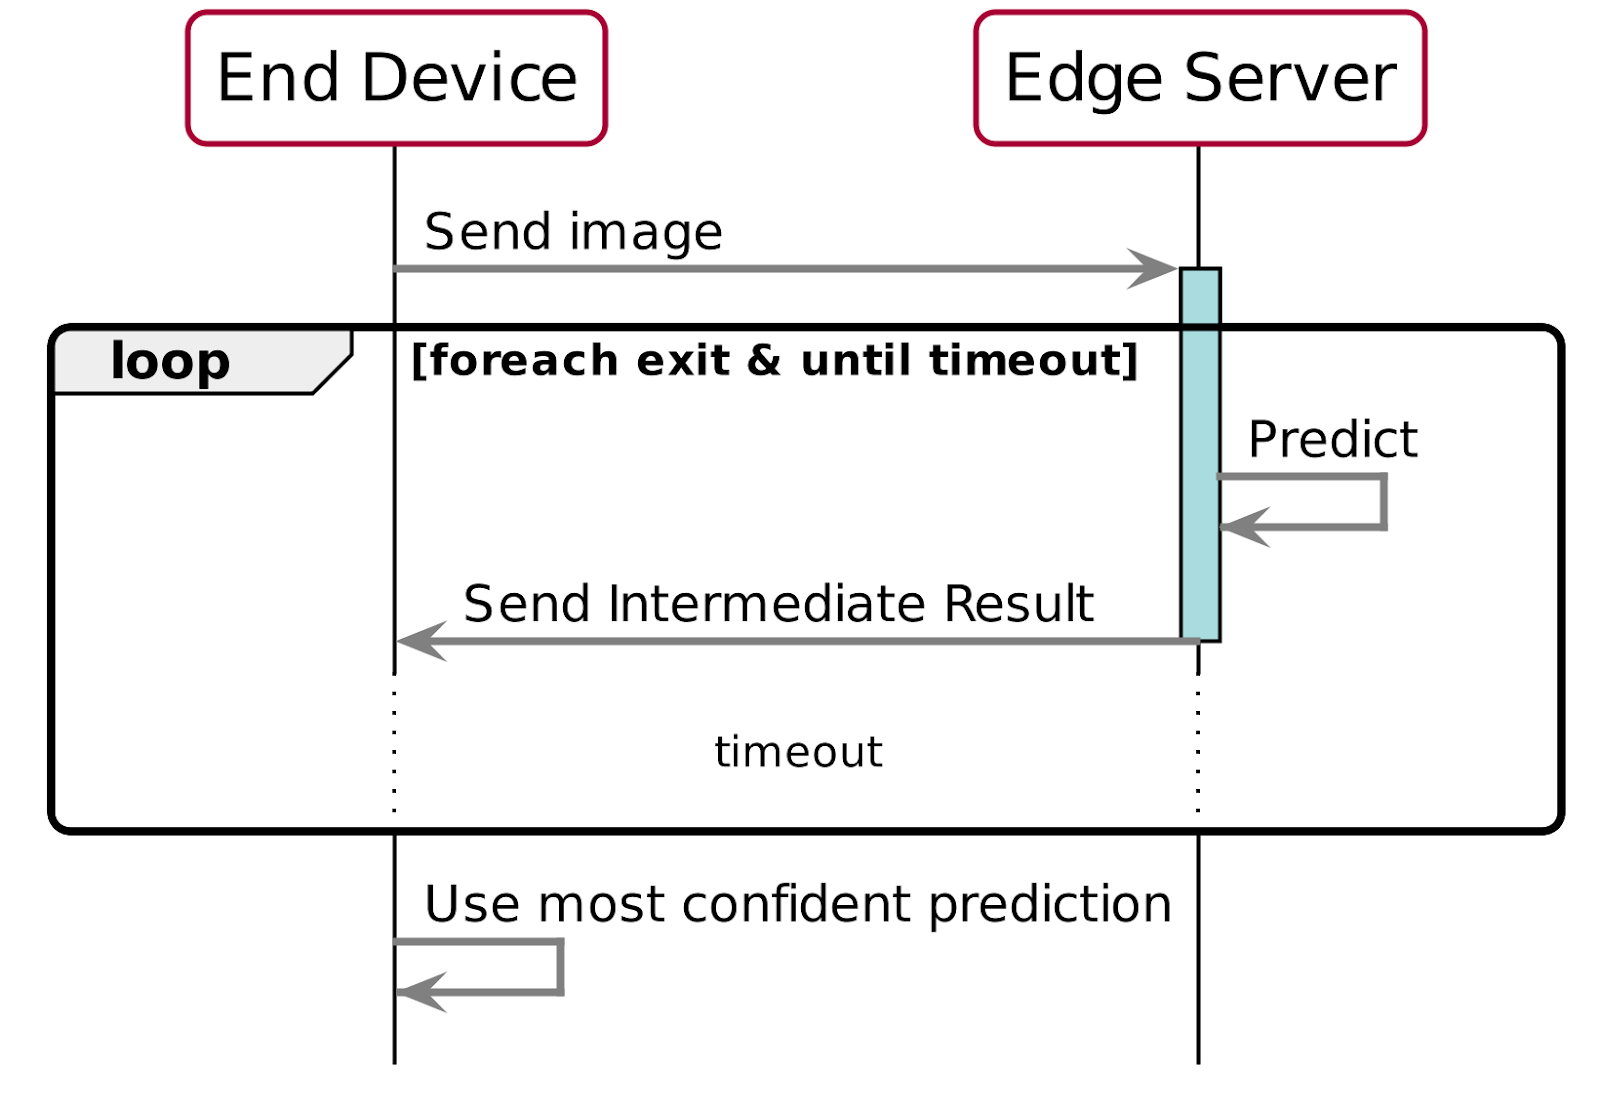
\includegraphics[width=.7\linewidth]{figures/models/sequence_diagram}
	\caption[Application Sequence Diagram]{Application Sequence Diagram}
	\label{fig:sequence-diagram}
\end{figure}

The implementation is written in \gls{python} using the \gls{python} Socket API \cite{noauthor_socket_nodate}. The client and server establishes a TCP socket connection. The client loads a samples from the \gls{min100} validation set, and streams the sample to the server. The server preprocess the sample and runs the model inference. As soon as, prediction are obtained, a thread is spawned, to stream the results back to the end device. 

The client is deployed on the \gls{nuc} and server on \gls{jetson} and \gls{gpu-ws}. The servers are LAN connected to the router and the client is connected over the WLAN.

\paragraph{Information Combination}

We send back the top-5 predictions to allow info-combination and reduce the data size of the reply. We use top-5, since the correct class is within these 5 predictions close to 90 \% of the time having just two predictions available for any of the models, see figure \ref{fig:top-5-cumulative}.

To combine top-5 prediction information from $ n $ exits, we must expand the vectors back to the original class space of $ C $ dimensions.

Each exit outputs two 5-dimensional vectors. $\mathbf{c}_{i,k}^{top5}$ contains the labels of the top-5 predictions and $ \mathbf{\hat{y}}_{i,k}^{top5}$ contain the class scores of the top-5 predictions. 

\begin{align}
\begin{split}
\mathbf{c}_{i,n}^{top5} &= \begin{bmatrix}
c_{i,n}^{1st} & \phantom{.}c_{i,n}^{2nd} & \phantom{.}c_{i,n}^{3rd} & \phantom{.}c_{i,n}^{4th} & \phantom{.}c_{i,n}^{5th}
\end{bmatrix}, \\
\mathbf{\hat{y}}^{top5}_{i,n} &= \begin{bmatrix}
\hat{y}_{i,n}^{1st} & \hat{y}_{i,n}^{2nd} & \hat{y}_{i,n}^{3rd} & \hat{y}_{i,n}^{4th} & \hat{y}_{i,n}^{5th}
\end{bmatrix}
\end{split}
\end{align}

The vectors are sorted from highest to lowest, hence the score $ \hat{y}_{i,k}^{1st} $ is associated the class label $ c_{i,k}^{1st} $ etc. 

We define an expansion function, which takes the top-5 score vector $ \mathbf{\hat{y}}_{i,n}^{top5}$ and top-5 class label vector  $\mathbf{c}_{i,n}^{top5}$ as input  $ f_{expand}\left(\bm{\hat{y}}_{i,n}^{top5},\mathbf{c}_{i,n}^{top5}\right) $ and outputs a $ C $-dimensional score vector, with the scores value at corresponding class index of the label vector, with the remaining indices are zero.
\begin{align}
f_{expand}\left(\bm{\hat{y}}_{i,n}^{top5},\mathbf{c}_{i,n}^{top5}\right) = 
\begin{bmatrix}
\hat{y}_{i,n,1} & \hat{y}_{i,n,2} & \hat{y}_{i,n,c} & \dots & \hat{y}_{i,n,C}
\end{bmatrix}_{1 \times C}
\end{align}
\todo{is this implementation?}

\subparagraph{Example: Expansion of a 10 class problem} 
\blockquote[]{	 	
	For this classification example, the number of classes $C=10$. From a prediction we get the two output vectors $\mathbf{l}_{i,n}^{top5}$ and $ \mathbf{\hat{y}}_{i,n}^{top5}$.
	\begin{align*}
	\mathbf{c}_{i,n}^{top5} &= \begin{bmatrix}
	\phantom{0}0\phantom{.0} & \phantom{0}3\phantom{.0} & \phantom{0}6\phantom{.0} & \phantom{0}8\phantom{.0} & \phantom{0}9\phantom{.0}
	\end{bmatrix},\\
	\mathbf{\hat{y}}_{i,n}^{top5} &= \begin{bmatrix}
	0.80 & 0.10 & 0.05 & 0.03 & 0.01
	\end{bmatrix}
	\end{align*}
	We use our expansion function $ f_{expand}\left(\bm{\hat{y}}_{i,n}^{top5},\mathbf{c}_{i,n}^{top5}\right) $, which return the score vector $ \mathbf{\hat{y}}_{i,n}$.
	\begin{align*}
	\mathbf{c}_{i,n} &= \begin{bmatrix}
	\phantom{0}0\phantom{.0} & \phantom{0}1\phantom{.0} & \phantom{0}2\phantom{.0} & \phantom{0}3\phantom{.0} & \phantom{0}4\phantom{.0} & \phantom{0}5\phantom{.0} & \phantom{0}6\phantom{.0} & \phantom{0}7\phantom{.0} & \phantom{0}8\phantom{.0} & \phantom{0}9\phantom{.0}
	\end{bmatrix}_{1 \times 10},\\
	\mathbf{\hat{y}}_{i,n}  &= \begin{bmatrix}
	0.80 & 0.00 & 0.00 & 0.10 & 0.00 & 0.00 & 0.05 & 0.00 & 0.03 & 0.01
	\end{bmatrix}_{1 \times 10}
	\end{align*}
}      

\section{Results} \label{sec:edge-results}

We want to examine the possibility to combine predictions from multiple exits to obtain a higher accuracy. A study of predictions results from all exits, revealed that in some cases an early exit correctly predicts a sample, which a later exit makes wrong. An example is sample 6 from the B-\gls{resnet}, $ y_6 $ is the ground truth, $ s^*_6 $ is the maximum score vector at each exit. $ k $ denotes the correctness of each exit as a binary value, where 1 is correct 0 is incorrect.
\begin{align*}
y_6=0,
\mathbf{l}_{6}=
\begin{bmatrix}
0 \\
54 \\
62 \\
62
\end{bmatrix},
\mathbf{s}^{*}_{6}=
\begin{bmatrix}
0.56 \\
0.32 \\
0.52 \\
0.62
\end{bmatrix},
\mathbf{k}_{6}=
\begin{bmatrix}
1 \\
0 \\
0 \\
0
\end{bmatrix}
\end{align*}
Based on the scores the models is more confident about the last exit prediction, even though the prediction from the first exit is correct. Having all predictions available using the combination functions Latest, max and add will all give the label 62, hence cherry-picking the correct prediction from this set of predictions, is not trivial. Analyzing the exit score have shown, that the score of a later exit is not always higher than the earlier exits, see figure \ref{fig:exit-highscore}. This phenomenon is named \emph{overthinking} in \cite{kaya_shallow-deep_nodate}.

\begin{figure}
	\captionsetup[subfigure]{justification=centering}
	\centering
	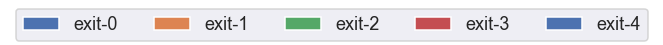
\includegraphics[width=.7\linewidth]{figures/edge/exit0-4_legend}
	\subfloat[B-ResNet]{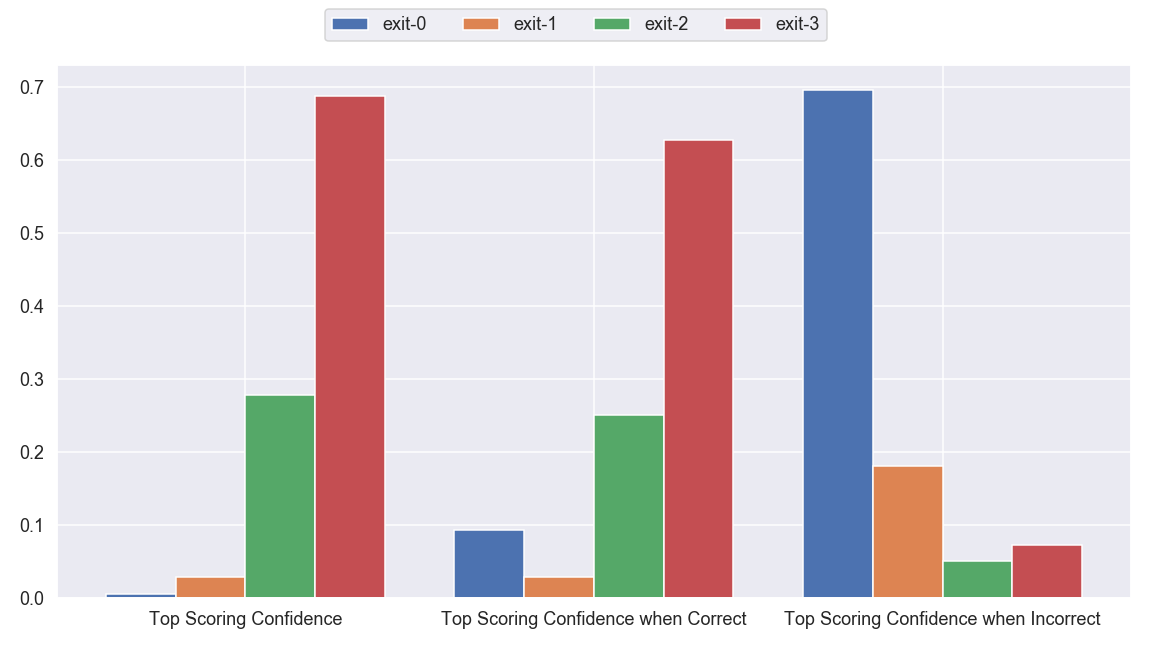
\includegraphics[width=.33\linewidth]{figures/edge/b-resnet_correctness}}
	\hfill
	\subfloat[B-DenseNet]{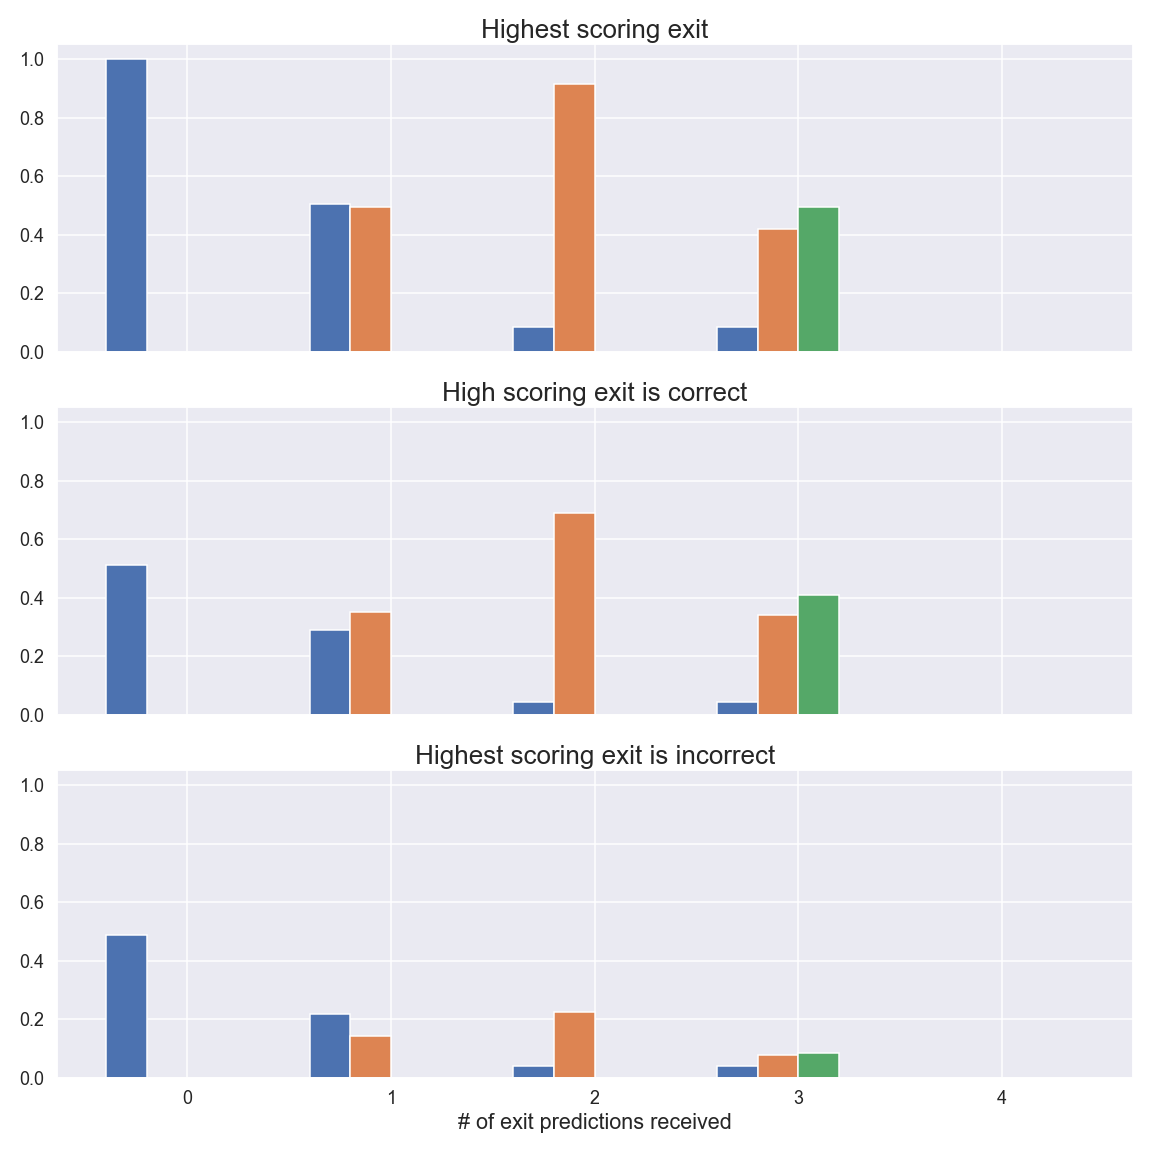
\includegraphics[width=.33\linewidth]{figures/edge/b-densenet_correctness}}
	\hfill
	\subfloat[MSDNet]{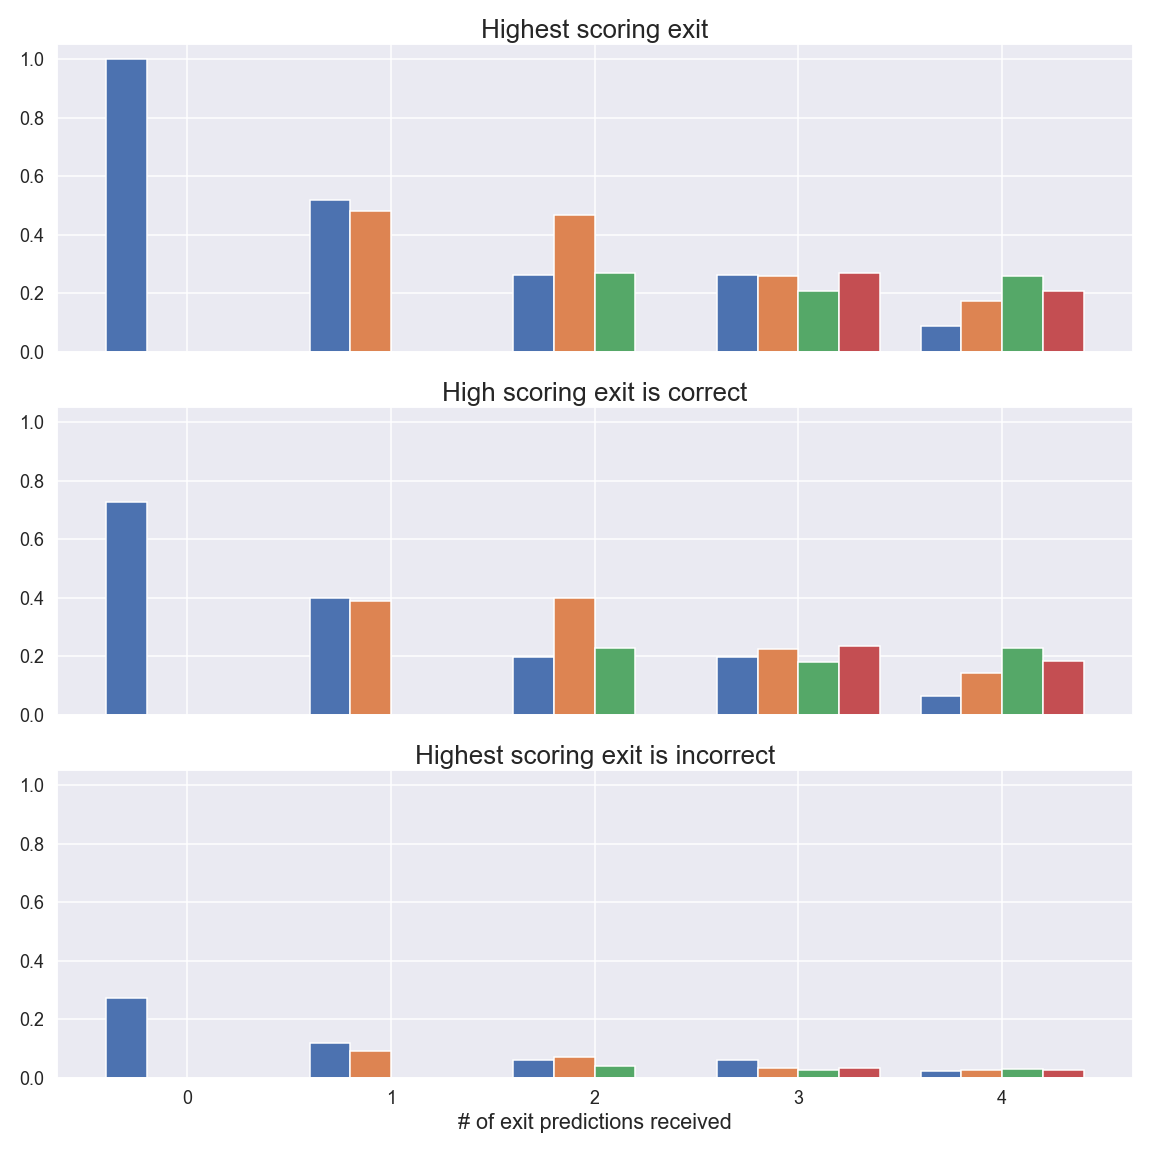
\includegraphics[width=.33\linewidth]{figures/edge/msdnet_correctness}}
	\caption[Model Highest Scoring Exit]{Model Highest Scoring Exit}
	\label{fig:exit-highscore}
\end{figure}

In fact, using the maximum score reduces the accuracy of the model, see table \ref{tbl:latest-vs-max}. It seems, that although the early exits achieve a higher score, they also introduces more uncertainty.  

\begin{longtabu}{>{\bfseries}X|X|X}
	\caption[]{} \label{tbl:latest-vs-max} \\
	\toprule
	\rowfont{\bfseries}
	Model & latest exit & max score   \tabularnewline
	\bottomrule
	\endfirsthead
	\multicolumn{3}{@{}l}{\textbf{\textcolor{black}{Table \ref{}:}} continued}\\
	\toprule
	\rowfont{\bfseries}
	Model & $Exit_N$ & max score    \tabularnewline
	\bottomrule
	\endhead % all the lines above this will be repeated on every page
	\bottomrule
	\multicolumn{3}{@{}l}{continued \ldots}\\
	\endfoot
	\hline
	\endlastfoot
	B-Resnet	& 0.8826	& 0.8794  \tabularnewline
	\hline
	B-DenseNet	& 0.8660 	& 0.8602 \tabularnewline
	\hline
	MSDNet		& 0.8640 	& 0.8598 \tabularnewline							
	\bottomrule
\end{longtabu}

Figure \ref{fig:exit-highscore} shows the distribution of highest scoring exit given the amount of prediction received, and whether the the highest score is correctly and incorrectly classified. The question is, if using top-5 scores from each exit, we can combine the scores to more confidently selecting the correct prediction among, to obtain a higher accuracy. Figure \ref{fig:top-5-cumulative} plots the top-5 accuracy against a cumulative top-5, that contains the top-5 from all previous exits. 

\begin{figure}
	\centering
	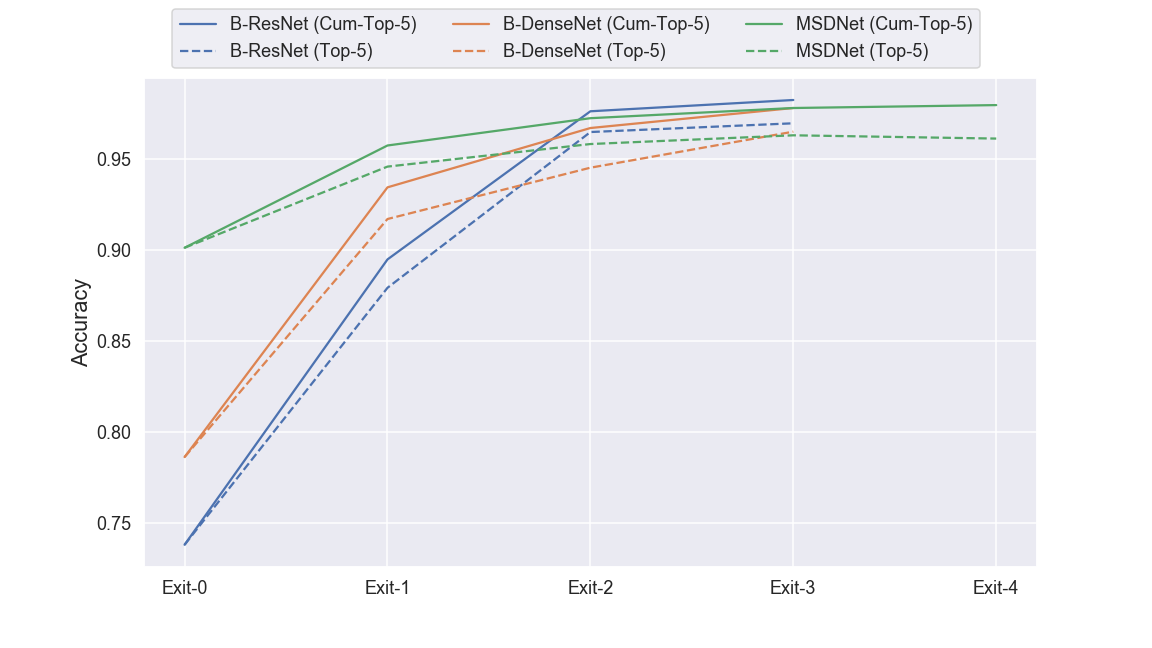
\includegraphics[width=.8\linewidth]{figures/edge/top5cumulative}
	\caption[Top-5 Cumulative]{Model Cumulative Top-5 Accuracy}
	\label{fig:top-5-cumulative}
\end{figure}

From the figure we can tell, that having multiple predictions does indeed improve the cumulative top-5. In the next section we apply the information combination functions to data obtain from running the early exit model and collecting the output scores. 

\subsection{Theoretical Information Combination Analysis}

Using the defined methods to combine the prediction information from multiple exits, as efforts to improve the overall model accuracy, is shown in figure \ref{fig:theoretical-info-combi}. The figure shows the obtainable accuracy given the number of exit predictions received. The blue line \textit{optimum-top5} show the maximum achievable accuracy, if we were always able to pick the right class among the cumulative top-5. The orange line, \textit{optimum-top1}, show the optimal line if, we were always able to pick the correct class among the cumulative top-1 predictions. None of the propose combination methods are able to improve the accuracy, when predictions from all exits is not available. Only the MSDNet shows a small improvement when adding predictions score, when all predictions are available.

\begin{figure}
	\captionsetup[subfigure]{justification=centering,farskip=1pt,captionskip=1pt}
	\centering
	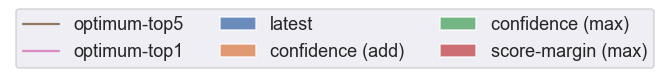
\includegraphics[width=.7\linewidth, keepaspectratio]{figures/edge/theoretical_score_combination_legend}
	\subfloat[B-ResNet]{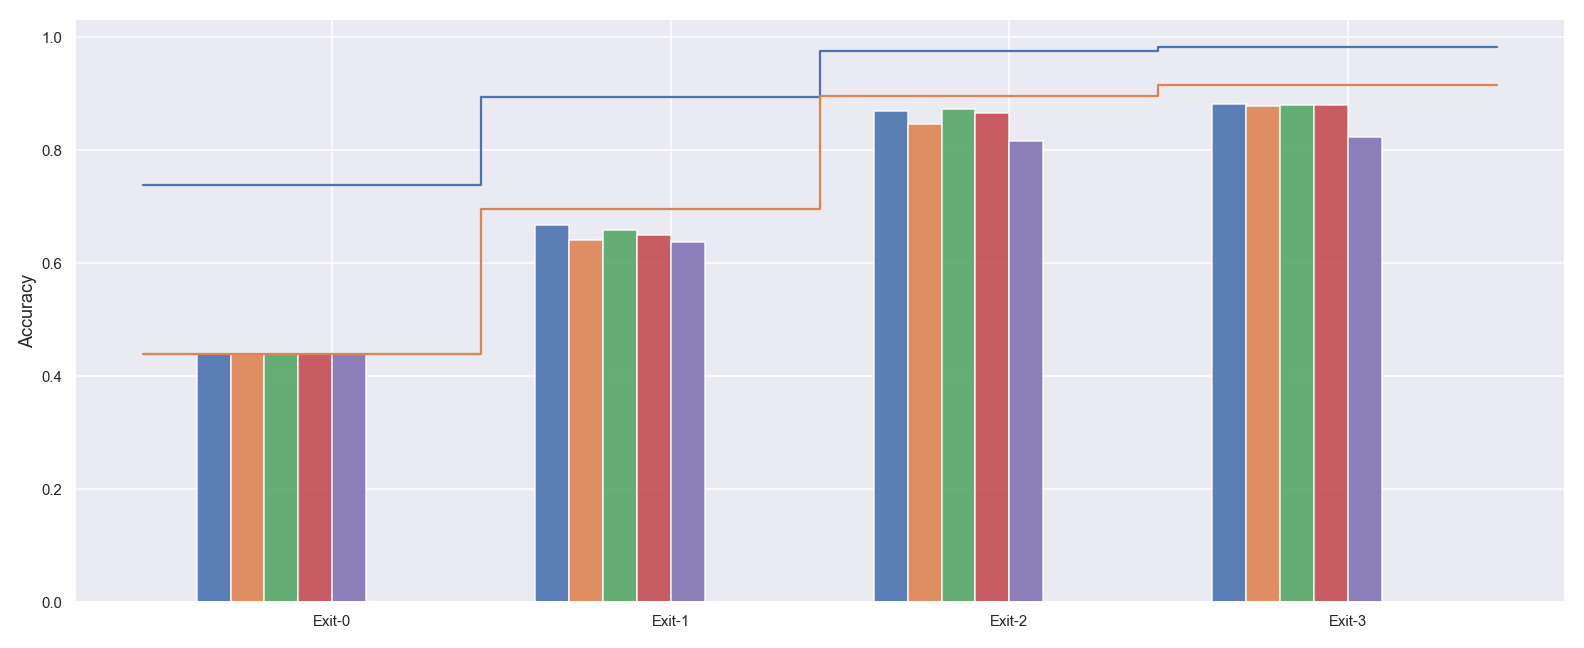
\includegraphics[height=.22\textheight, keepaspectratio]{figures/edge/b-resnet_theoretical_score_combinations}}
	\hfill
	\subfloat[B-DenseNet]{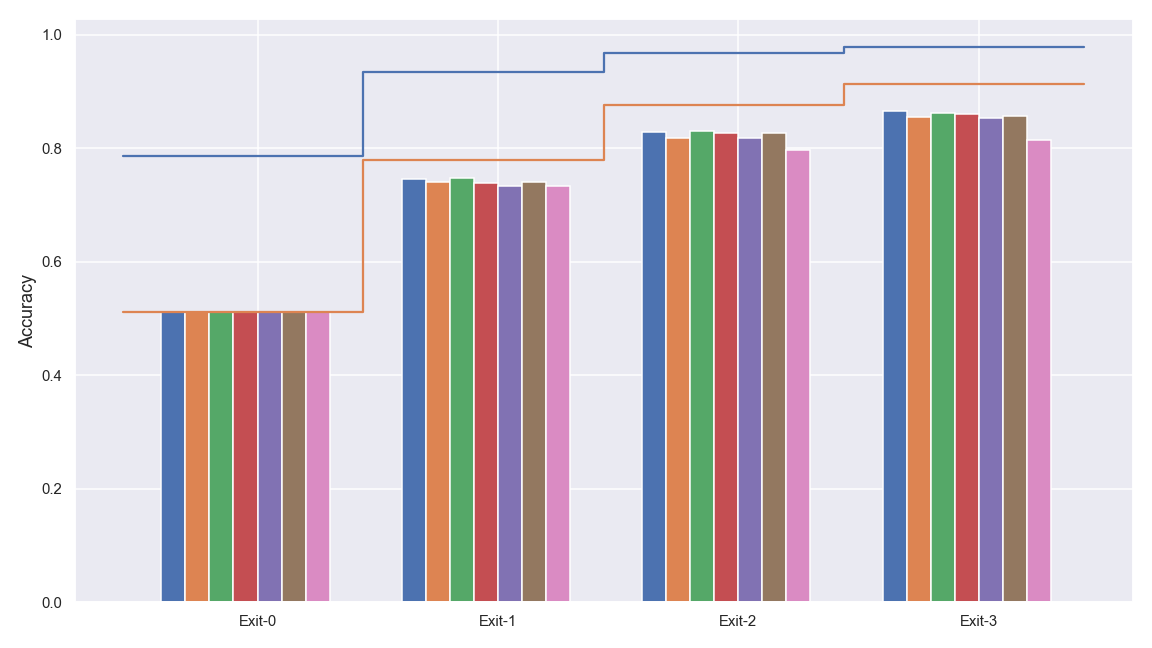
\includegraphics[height=.22\textheight, keepaspectratio]{figures/edge/b-densenet_theoretical_score_combinations}}
	\hfill
	\subfloat[MSDNet]{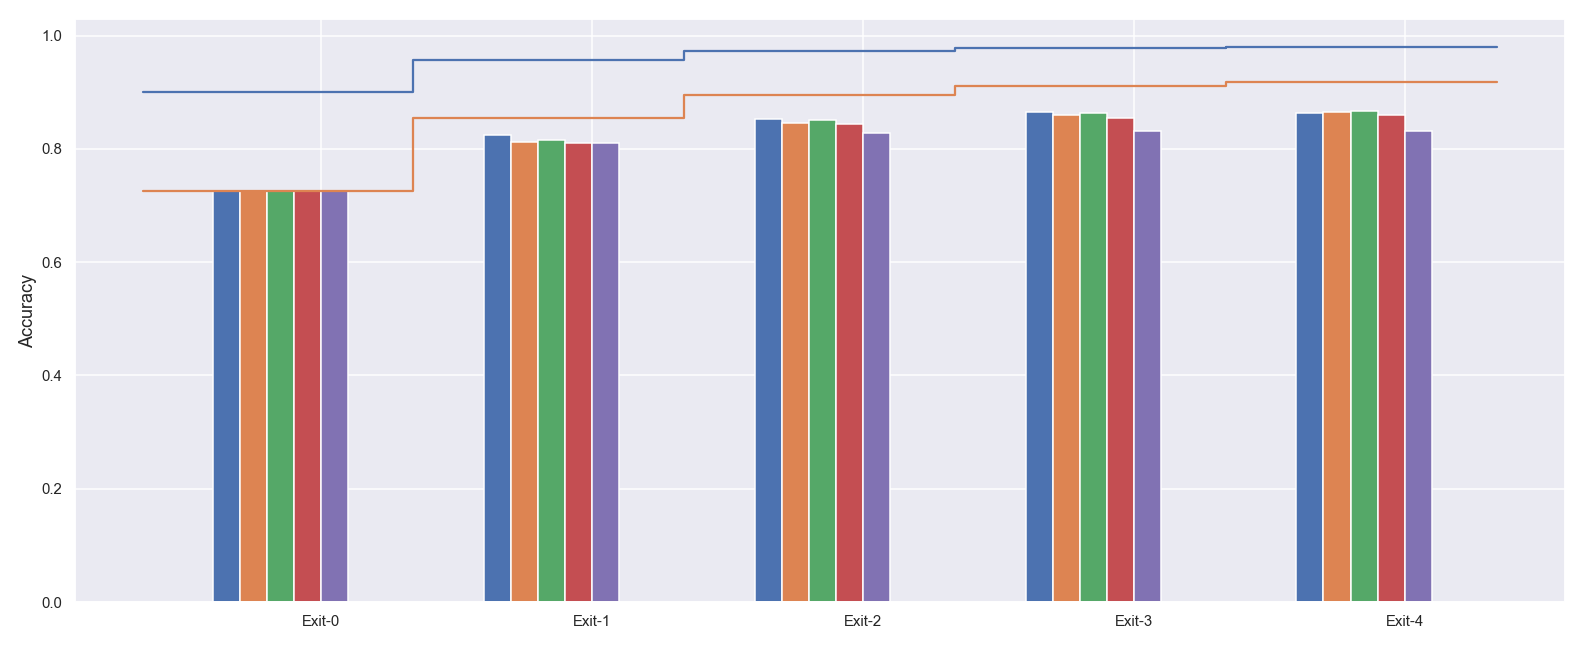
\includegraphics[height=.22\textheight, keepaspectratio]{figures/edge/msdnet_theoretical_score_combinations}}
	\caption[Combination Function with $ n $ Available Exits]{Combination Function with $ n $ Available Exits}
	\label{fig:theoretical-info-combi}
\end{figure}



\subsection{Edge Offloading: \gls{aee} vs Conventional Offloading}

We run test where the images are offloaded from NUC to Jetson. We set different delay threshold and plot the achievable reliability using the prediction from the latest exit, see figure \ref{fig:practical-offloading}. If we compare with figure \ref{fig:delay-threshold}, we obtain less sharp steps, in the areas where a new exit begin to be obtainable, due to the added deviation from the communication. Given this figure, we can select the proper model under different delay threshold, be always selecting the model achieving the highest reliability.  

\begin{figure}
	\captionsetup[subfigure]{justification=centering,farskip=1pt,captionskip=1pt}
	\centering
	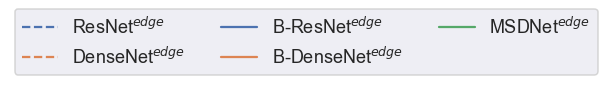
\includegraphics[width=.5\linewidth]{figures/edge/offloading_legend}
	\subfloat[\gls{jetson}]{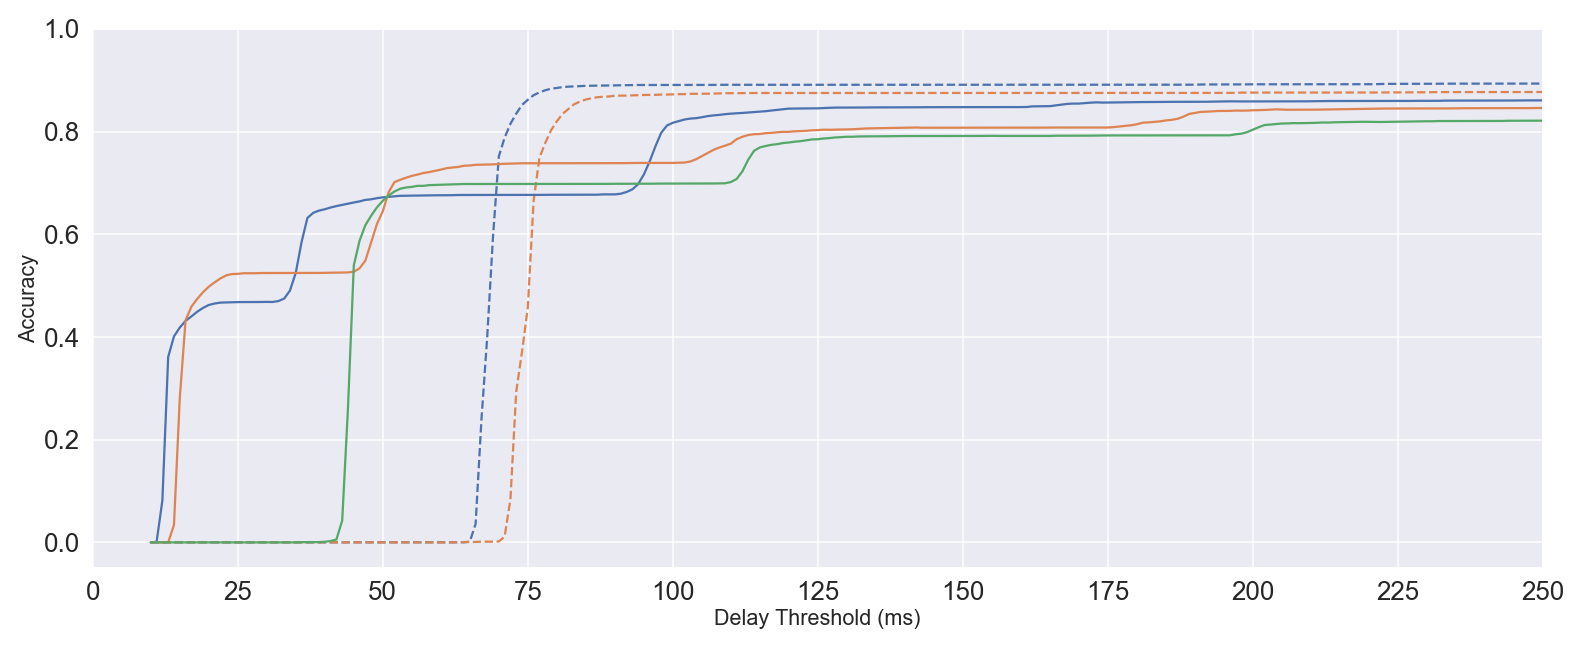
\includegraphics[width=.8\linewidth]{figures/edge/jetson_offloading}}
	\hfill
	\subfloat[\gls{gpu-ws}]{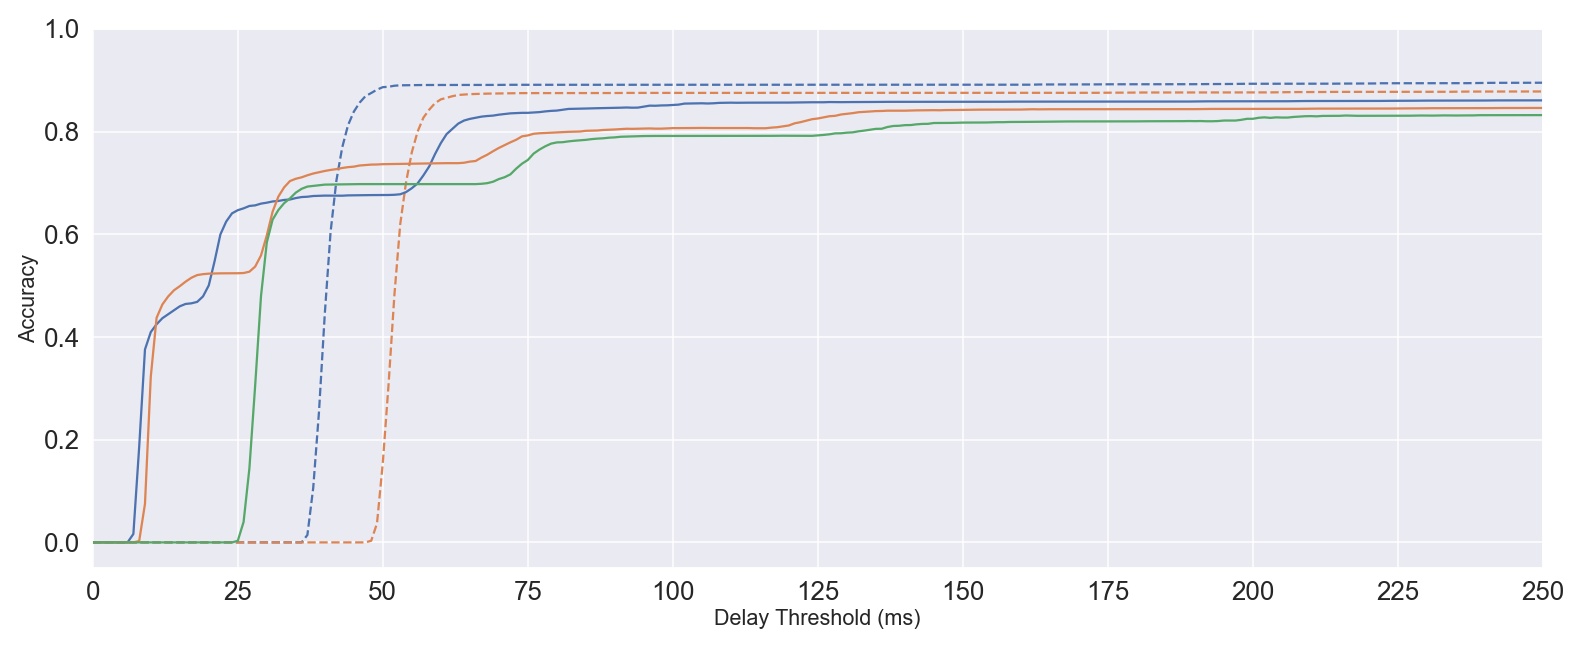
\includegraphics[width=.8\linewidth]{figures/edge/gpu_offloading}}
%	\subfloat[Local Jetson TX2]{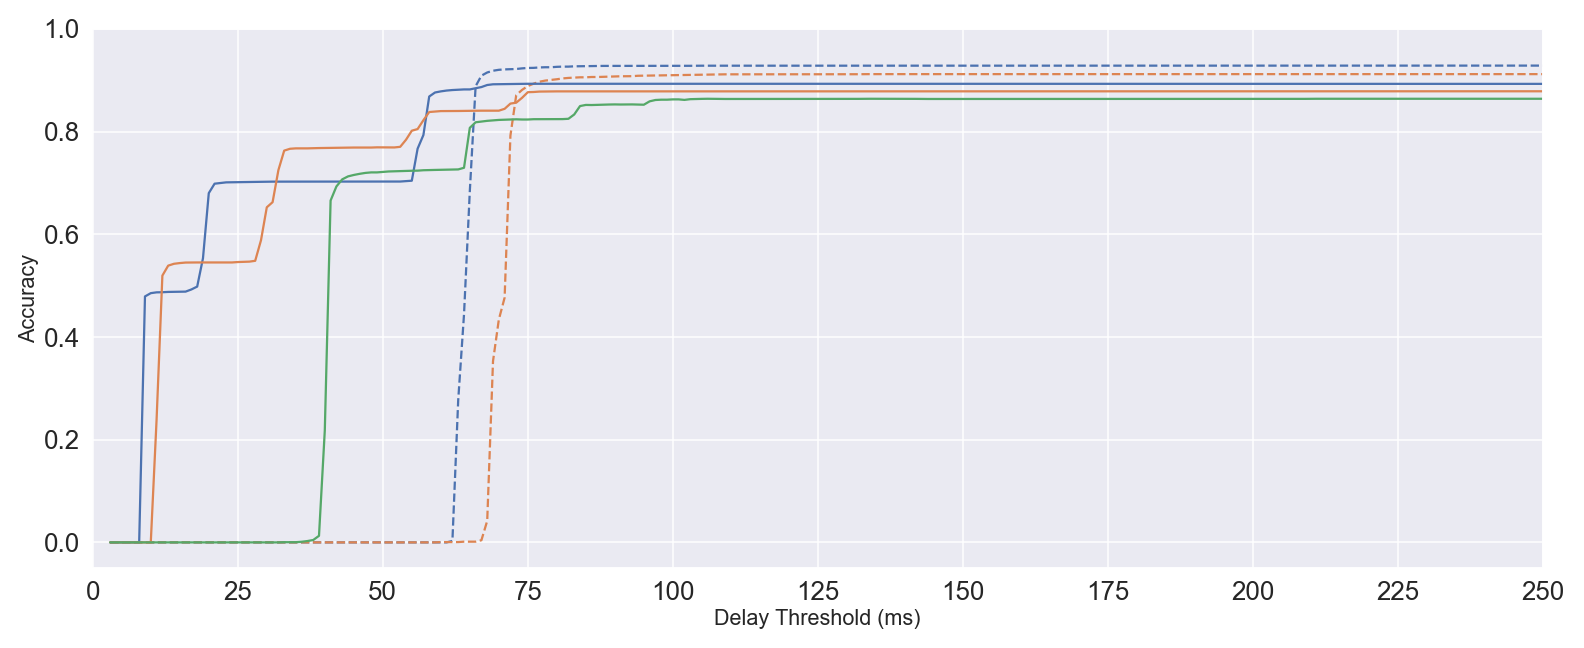
\includegraphics[width=\linewidth]{figures/delay_plots/jetson__delay_threshold}}
	\caption[Offloading NUC to Jetson]{Offloading NUC to Jetson}
	\label{fig:practical-offloading}
\end{figure}

In table \ref{tbl:time-offloading} we present the measured communication time stats, mean, standard deviation, minimum- and maximum value. From the table we see the largest deviation, which support our assertion of the softer steps.  

\begin{longtabu}{>{\bfseries}X|X|X|X|X}
	\caption[]{} \label{tbl:time-offloading} \\
	\toprule
	\rowfont{\bfseries}
	 & \multicolumn4{c}{Communication Time (ms)}    \tabularnewline
	 \tabucline{2-5}
	\rowfont{\bfseries} Offloading & Mean & Std. & Min & Max   \tabularnewline
	\bottomrule
	\endfirsthead
	\multicolumn{3}{@{}l}{\textbf{\textcolor{black}{Table \ref{tbl:time-offloading}:}} continued}\\
	\toprule
	\rowfont{\bfseries}
	Offloading & Up- and downlink Communication Time (ms) &    \tabularnewline
	\bottomrule
	\endhead % all the lines above this will be repeated on every page
	\bottomrule
	\multicolumn{3}{@{}l}{continued \ldots}\\
	\endfoot
	\hline
	\endlastfoot
	NUC to Jetson	& 25.68	& 110.93 & 2.35 & 962.76  \tabularnewline						
	\bottomrule
\end{longtabu}

Additionally, we made a measurement of the delay using the reliable transport protocol, \gls{tcp}. In figure \ref{fig:tcp-overhead}, one can see the impact of using \gls{tcp}. In the three different settings (meetingroom, kitchen, and kitchen) the end-device is moved further apart, which reduced the quality of the communication link. In poor communication environment \gls{tcp} can be expected to have a high overhead introduced by required retransmission, thus have a negative impact on the overall delay.  

\begin{figure}
	\centering
	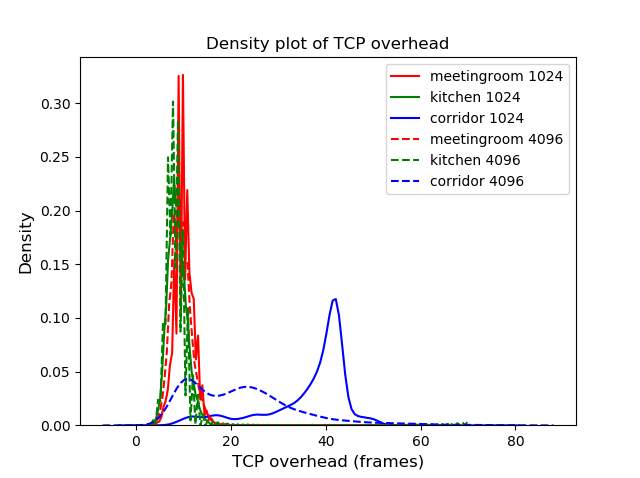
\includegraphics[width=.75\linewidth]{figures/tcp/tcpoverhead}
	\caption[TCP retransmission overhead]{TCP retransmission overhead}
	\label{fig:tcp-overhead}
\end{figure}

We compare running the various model locally on the NUC with offloading to the Jetson, see figure \ref{fig:offloading-vs-local}. Especially under stringent delay thresholds, i.e. the lower region of the plots, we are able to improve the accuracy significantly. However, as the delay threshold are relaxed running locally becomes preferable. One may notice the small drop in reliability, these are cause by extreme delays in the \gls{tcp} protocol, that does not occur locally.

We have conducted experiment with using both \gls{jetson} and \gls{gpu-ws} as edge servers and \gls{nuc} as end device. We compare edge offloading the different models across the two edge platforms and with local inference on the \gls{nuc}. In figure \ref{fig:resnet-offloading-vs-local} we compare the \gls{resnet} based models. In figure \ref{fig:densenet-offloading-vs-local} the \gls{densenet} based models and lastly in figure \ref{fig:msdnet-offloading-vs-local} the \gls{msdnet} model.

\begin{figure}
	\captionsetup[subfigure]{justification=centering, farskip=0pt,captionskip=0pt}
	\centering
	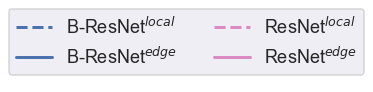
\includegraphics[width=.3\linewidth]{figures/edge/gpu_b-resnet_offloading_vs_local_legend}
	\hfill
	\subfloat[GPU Workstation as Edge\label{fig:resnet-offloading-vs-local-jetson}]{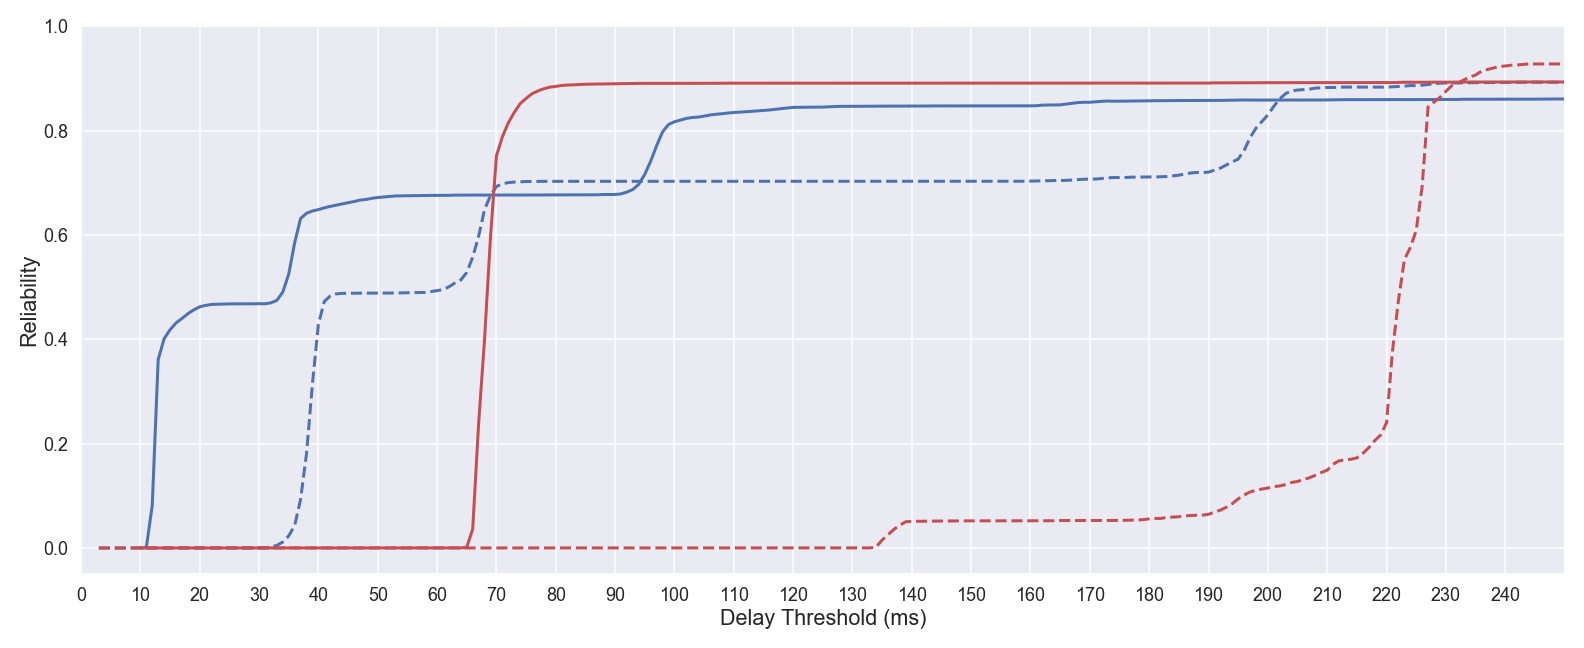
\includegraphics[width=\textwidth,height=.22\textheight,keepaspectratio]{figures/edge/jetson_b-resnet_offloading_vs_local}}
	\hfill
	\subfloat[GPU Workstation as Edge\label{fig:resnet-offloading-vs-local-gpu}]{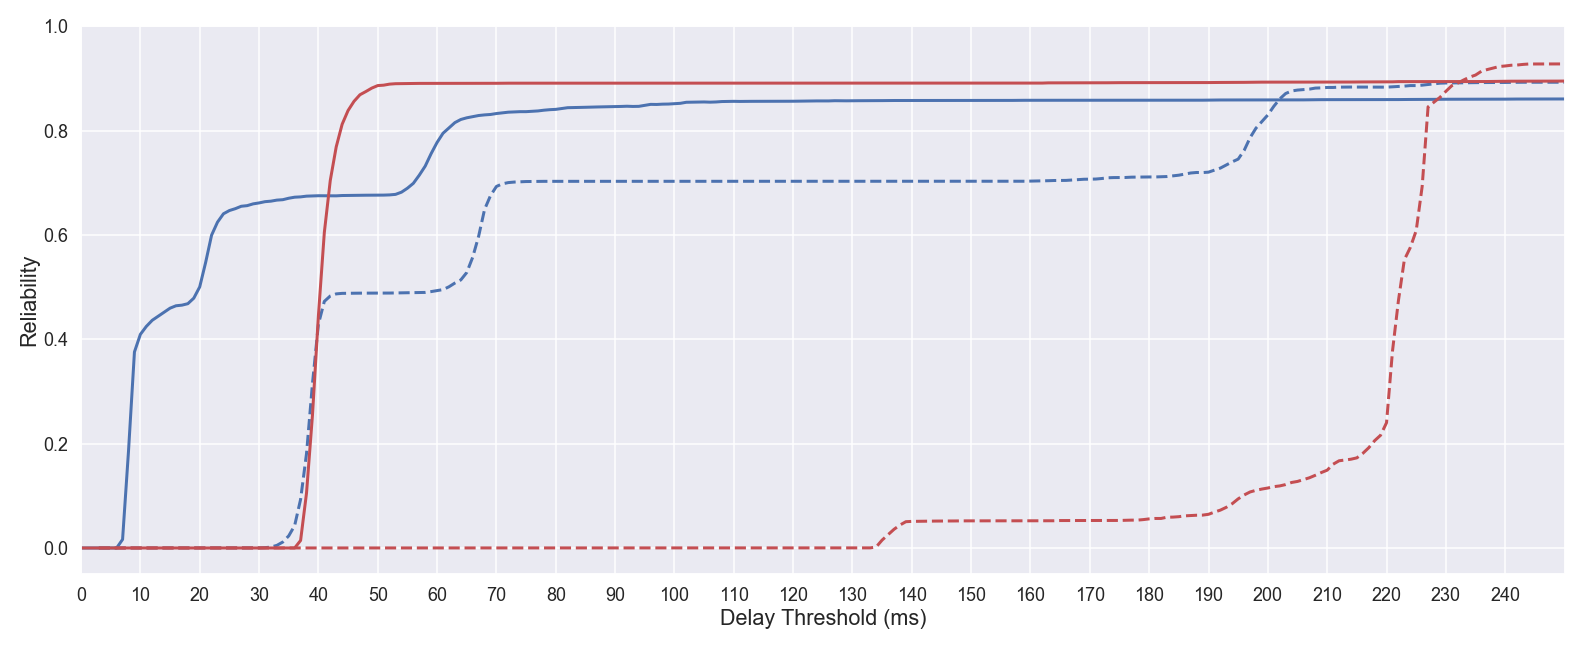
\includegraphics[width=\textwidth,height=.22\textheight,keepaspectratio]{figures/edge/gpu_b-resnet_offloading_vs_local}}
	\caption[Offloading comparison of residual networks]{Offloading comparison of residual networks}
	\label{fig:resnet-offloading-vs-local}
\end{figure}

From figure \ref{fig:resnet-offloading-vs-local} we see, how we are able to improve the reliability under stringent delay requirement using either platform as edge server instead of local inference. We can also see, that we improve the reliability compared to using a conventional model again under stringent requirements. When offloading the conventional model, it starts to outperform the early exit model, if we have above 80ms available using the \gls{jetson} or 50ms available using the \gls{gpu-ws}. Local inference is the best option when having 250 ms available, which is we rarely have. The reason why local execution can obtain a higher reliability, is due to some samples are missed as they do not meet the deadline, this is mostly caused by variations in communication time. 

\begin{figure}
	\captionsetup[subfigure]{justification=centering, farskip=0pt,captionskip=0pt}
	\centering
	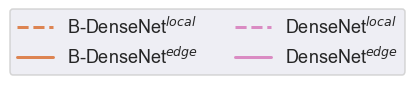
\includegraphics[width=.3\linewidth]{figures/edge/gpu_b-densenet_offloading_vs_local_legend}
	\hfill
	\subfloat[\gls{jetson} as Edge\label{fig:densenet-offloading-vs-local-jetson}]{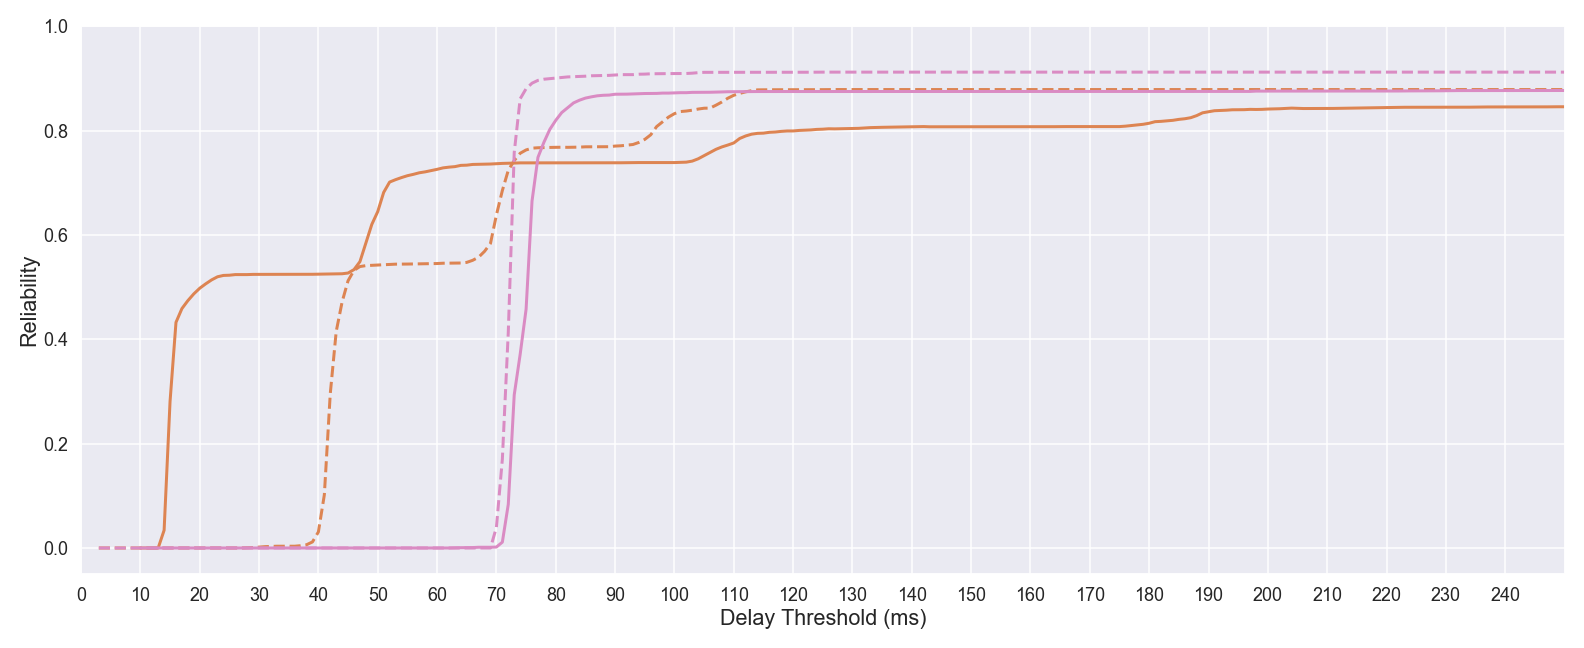
\includegraphics[width=\textwidth,height=.22\textheight,keepaspectratio]{figures/edge/jetson_b-densenet_offloading_vs_local}}
	\hfill
	\subfloat[GPU Workstation as Edge\label{fig:densenet-offloading-vs-local-gpu}]{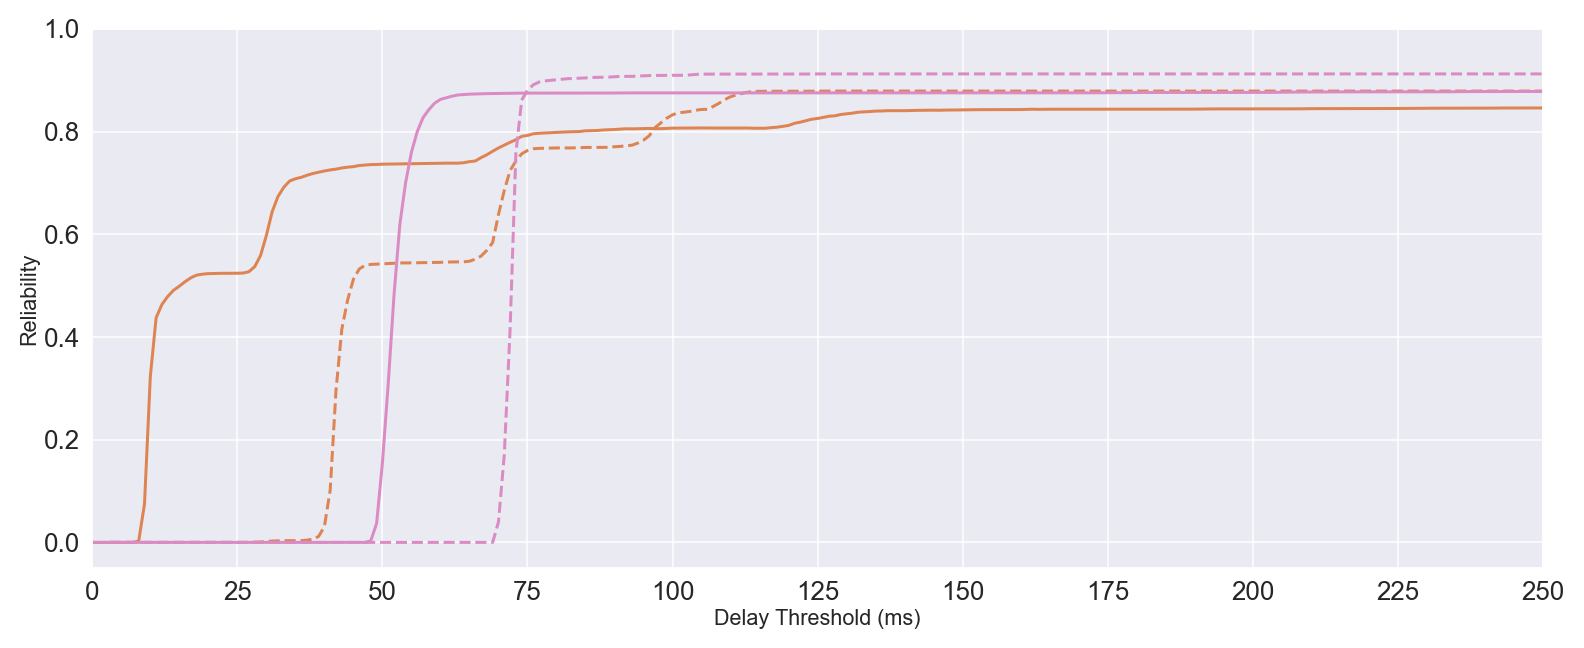
\includegraphics[width=\textwidth,height=.22\textheight,keepaspectratio]{figures/edge/gpu_b-densenet_offloading_vs_local}}
	\caption[Offloading comparison of densely connected networks]{Offloading comparison of densely connected networks}
	\label{fig:densenet-offloading-vs-local}
\end{figure}

The \gls{densenet} tells a somewhat different story. We are still able to improve reliability remarkably under stringent delay requirements using \gls{aee}, compared to offloading a conventional model or locally inference. However, when reaching 70-80 ms on \gls{jetson} all other schemes, local inference B-\gls{densenet} or \gls{densenet} and also offloading \gls{densenet}, starts to outperform \gls{aee}. Local inference of the conventional model is even faster than offloading. The performance difference between the \gls{jetson} and \gls{nuc} is not big enough for the \gls{densenet} based model, this we can tell from looking at \gls{gpu-ws}, where offloading is performing better under 75 ms. 

\begin{figure}
	\captionsetup[subfigure]{justification=centering, farskip=0pt,captionskip=0pt}
	\centering
	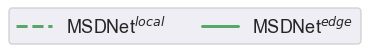
\includegraphics[width=.3\linewidth]{figures/edge/gpu_msdnet_offloading_vs_local_legend}
	\hfill
	\subfloat[GPU Workstation as Edge]{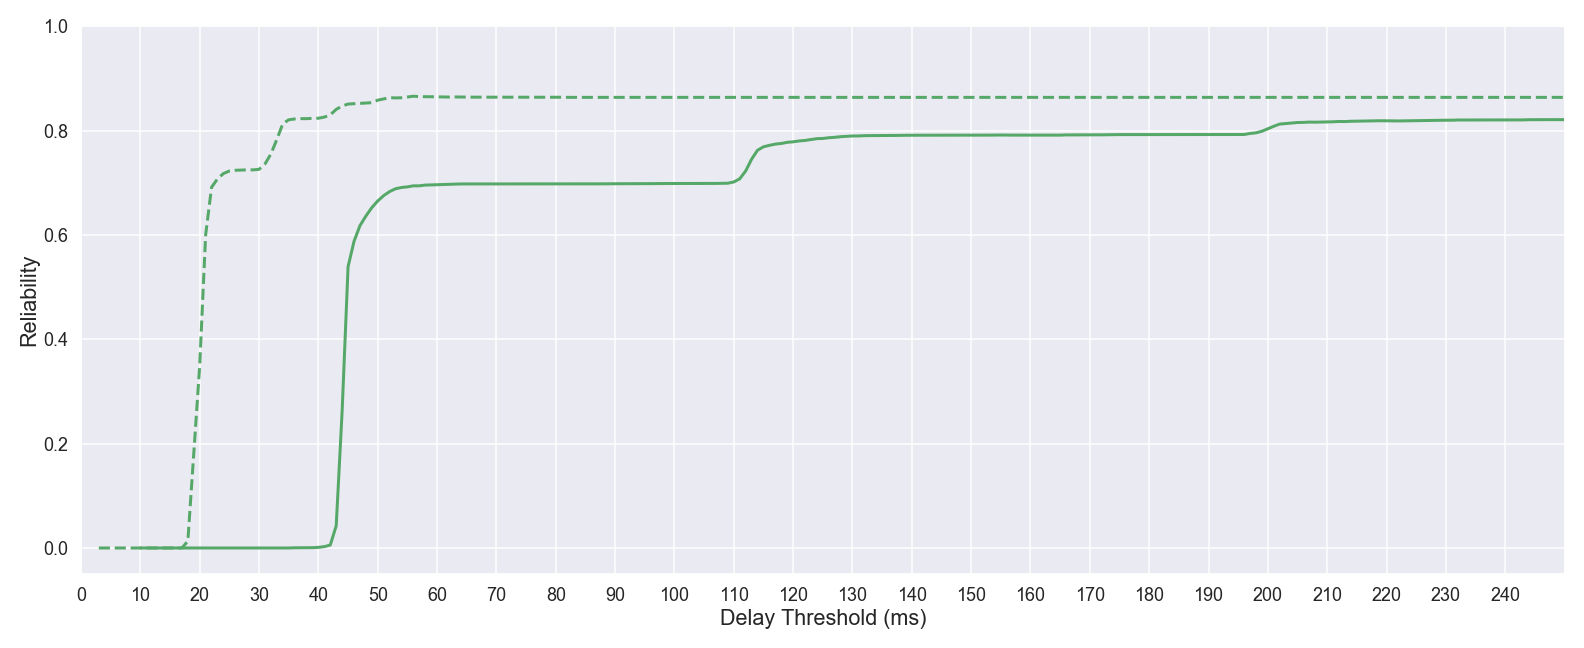
\includegraphics[width=\textwidth,height=.22\textheight,keepaspectratio]{figures/edge/jetson_msdnet_offloading_vs_local}}
	\hfill
	\subfloat[GPU Workstation as Edge]{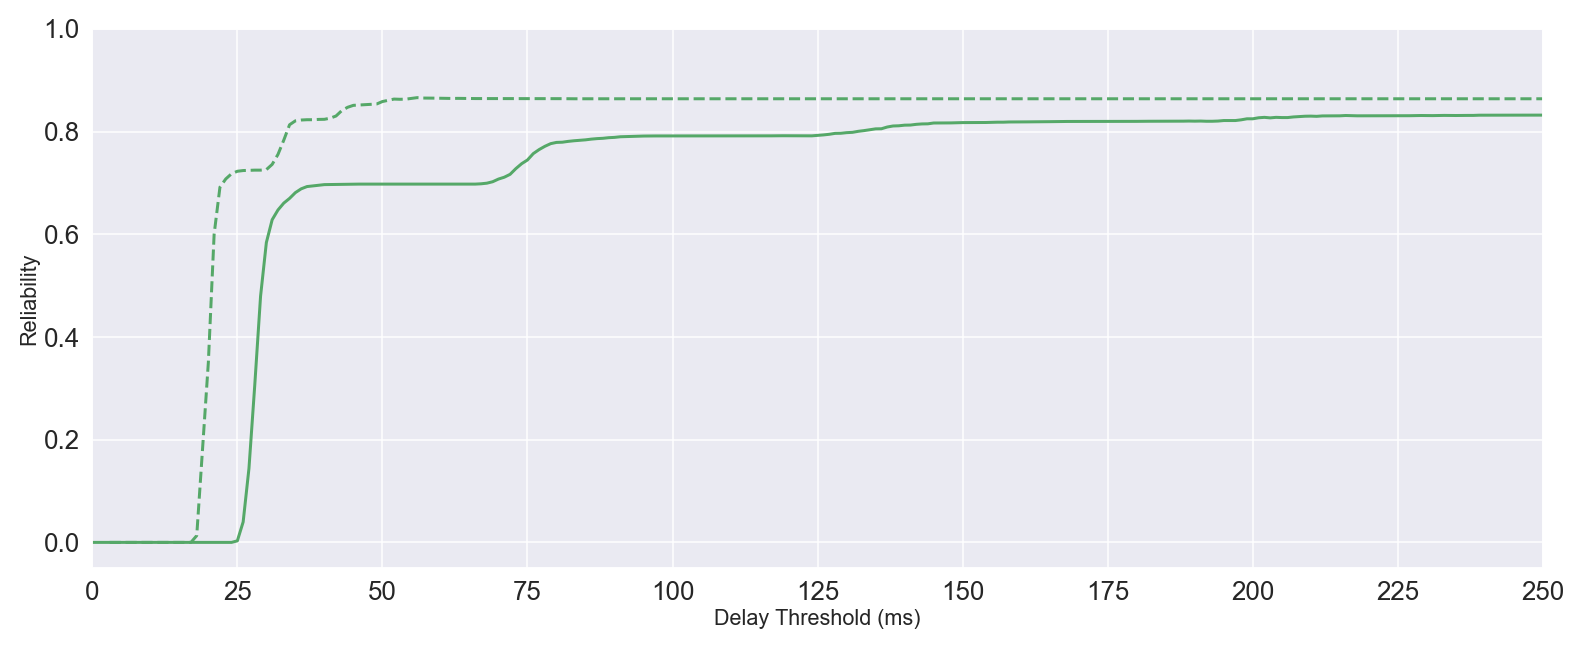
\includegraphics[width=\textwidth,height=.22\textheight,keepaspectratio]{figures/edge/gpu_msdnet_offloading_vs_local}}
	\caption[Offloading comparison of multi-scale dense networks]{Offloading comparison of multi-scale dense networks}
	\label{fig:msdnet-offloading-vs-local}
\end{figure}

\gls{msdnet} tells a completely different story. Local inference is always able to achieve higher reliability irregardless of offloading to \gls{jetson} or \gls{gpu-ws}. We do not elaborate on this tedency, as we saw the same tedency in chapter \ref{ch:earlyexit} and have already discussed it in section \ref{sec:ee-summary}.

\section{Summary} \label{sec:edge-summary}

In this section we summarize and discuss the results from previous section. We did not manage to come up with a combination function, that was able to improve the accuracy when only a few predictions were available, because the early exit prediction comes with a lot of uncertainty. Only for the \gls{msdnet} when predictions from all exit were present, we were able to improve the accuracy. The reason being, that all exits of this model produces decent prediction accuracy in general, hence less uncertainty from early exit. We have found, that using the latest received predictions, is the best overall for these early exit models.

We used this finding to set up a practical test of \gls{aee}, were images was sent from the NUC to the Jetson, thus introducing communication latency. We found, that we were able to improve the reliability for both B-\gls{resnet} and B-\gls{densenet} under stringent delay budget. However, for the \gls{msdnet} our offloading solution was uncompetitive with local execution. 

The NUC is a very powerful end device equipped with a \gls{cpu}. The end device are more likely to be equipped with ARM processors or even smaller processing unit. Some end devices may even not be able to run any of the models locally. However, given these results, the edge servers may not need to be equipped with powerful \gls{gpu}s, as the NUC is able to achieve such high performance running the \gls{msdnet}.

Comparing \gls{aee} with Edgent, where a selection of exit is based on regression models of inference time and a current state of bandwidth. Edgent will too suffer from unexpected communication delays, that simply is more uncertain than computation delays. Hence some predictions will be lost, as they will not be able to meet the latency requirement. Our solutions have higher probability of receiving just a single prediction, when a timeout occurs, where none is available for Edgent, if the prediction unexpectedly violates the deadline. 

Our solution is also applicable in collaborative edge, where the end-device locally processes the algorithm up to an early exit and obtains a prediction, then offloads the rest of the execution in a cascaded manner for remote execution, still if no reply is received from the edge within the time frame, a locally obtained prediction is available. Thus, the reliability of the solution is improved. However, this approach leads to idle time on server, when the first exit is processed locally on a less powerful device. The early layers of the \gls{dnn} is typically also the most demanding leading to worsened inference time. Additionally, communication of features from the earliest exits is also heavier than later layer and also heavier compared to sending the compressed image, if no network partition feature compression technique is used. This can indeed worsen the reliability, as less exit predictions are actually able to meet the deadline, when more latency is introduced to the solution.

Instead we have propose a solutions to handle the lost prediction dilemma. However, still only possible if local processing is an option. In a modified version of the Big/Little \gls{dnn}, where the end device offloads the compressed image to edge server and in parallel process a smaller and less accurate \gls{dnn} locally. The upside is, that the application can then always use the locally obtained prediction and choose to discard it, as more accurate prediction arrives from edge or if a good combination function is found use the information to choose the best prediction. If offloading is not an possible, then the \gls{aee} at the edge is the better option.

Edge/cloud offloading using current communication technologies, can potentially experience service outage. If an access point is no longer accessible, reconnection delays to a new or the same access point e.g. using WiFi can be expected to take at least 1s \cite{pei_why_2017}. Which will inevitably lead to lost predictions, if no local inference is feasible. In \cite{wang_see:_2019} a scheduling scheme is proposed to handle on device inference of early exit \gls{dnn}s, if experiencing service outages to offloading services.

The down-side of our approach is scheduling, if we encounter time-out in between to exits the computation is wasted, which could have been used to process the next frame. We introduce some pessimism, by letting the server known the deadline and measured bandwidth, the server measures the time it uses and can decide to terminate the inference process and continue with next frame, if the server already knowns, it cannot meet reach next exit, and deliver prediction results to the client before the deadline.

In conclusion of this chapter, we were able to improve the reliability, when using \gls{aee} to run early exit models (B-\gls{resnet} and B-\gls{densenet}) on the edge compared to on-device inference. We were not able to come up with a combination function to compete with the just using the prediction from the latest exit. 


In the next section we present work related to inference architecture. 

Edgent \cite{li_edge_2018} combines early exiting and network splitting to handle the accuracy-latency trade-off, by an optimization framework of \gls{dnn} right-sizing and splitting for device-edge collaboration. The optimization done based on regression models of the per layer execution time of the \gls{dnn}. We argue, that Edgent's upfront selection of exit i.e gls{dnn} right-sizing, does not account for unpredictable communication delays, that we try to address. 

Early exiting is proposed in . Early exit model is used in Edgent \cite{li_edge_2018} to investigate classification of real-time video streaming. They propose a partial offloading scheme for device/edge co-inference, using an optimizer to maximize the service accuracy while complying with latency requirements. Edgent uses model partitioning to find an optimal splitting point of the \gls{dnn} and model right-sizing to select an early exit point as final exit.

Their solution may suffer from sporadic unexpected communication delays or service outages under the inference process. We account for this by not selecting an exit point upfront, but uses all predictions we received prior to the deadline. In worst case the first exit is never reachable, hence neither \gls{aee}, nor Edgent will receive a prediction within the deadline. If the first exit is reachable \gls{aee} will always receive at least on prediction, whereas if Edgent selected a later exit, that turned out to not be reachable, no prediction is received in time. \todo{is this too much discussion and critique? Should i use it in justification of our design instead? as I sort of already do...}

In \cite{wang_see:_2019} \gls{see} is proposed. As the name implies, \gls{see} is a scheduling of early exit model for on-device inference.  \gls{see} also uses real-time video streaming as use case, by scheduling frames able to meet the deadline and  ignoring frames that cannot, to maximize the utility. We deem our solution could benefit from the scheduling of video frames, if is was to be extended to real-time video streaming. 

However, as the overhead of our early exit model's additional exits is negligible, we argue that using our optimistic scheme for edge inference, that always tries to deliver the best possible prediction before the deadline, would outperform upfront exit selection. Our scheme could easily be used in combination with \gls{see}, by switching to \gls{see} for on-device inference, when poor networking connection or service outage is detected. \todo{same}

In the next section the structure of the rest of the thesis presented
